\problemname{Ada Loveslaces}

A shoe has a lacing geometry: $N$, the number of eyelets (on a side), $d$,
the distance between eyelets, $s$, the separation between the columns of
eyelets when the shoe is laced, and $t$, the thickness of an eyelet.
In Figure 1 below, $N = 3$, with eyelets numbered from $0$ to $2N - 1$.
\begin{figure}[h]
	\begin{center}
		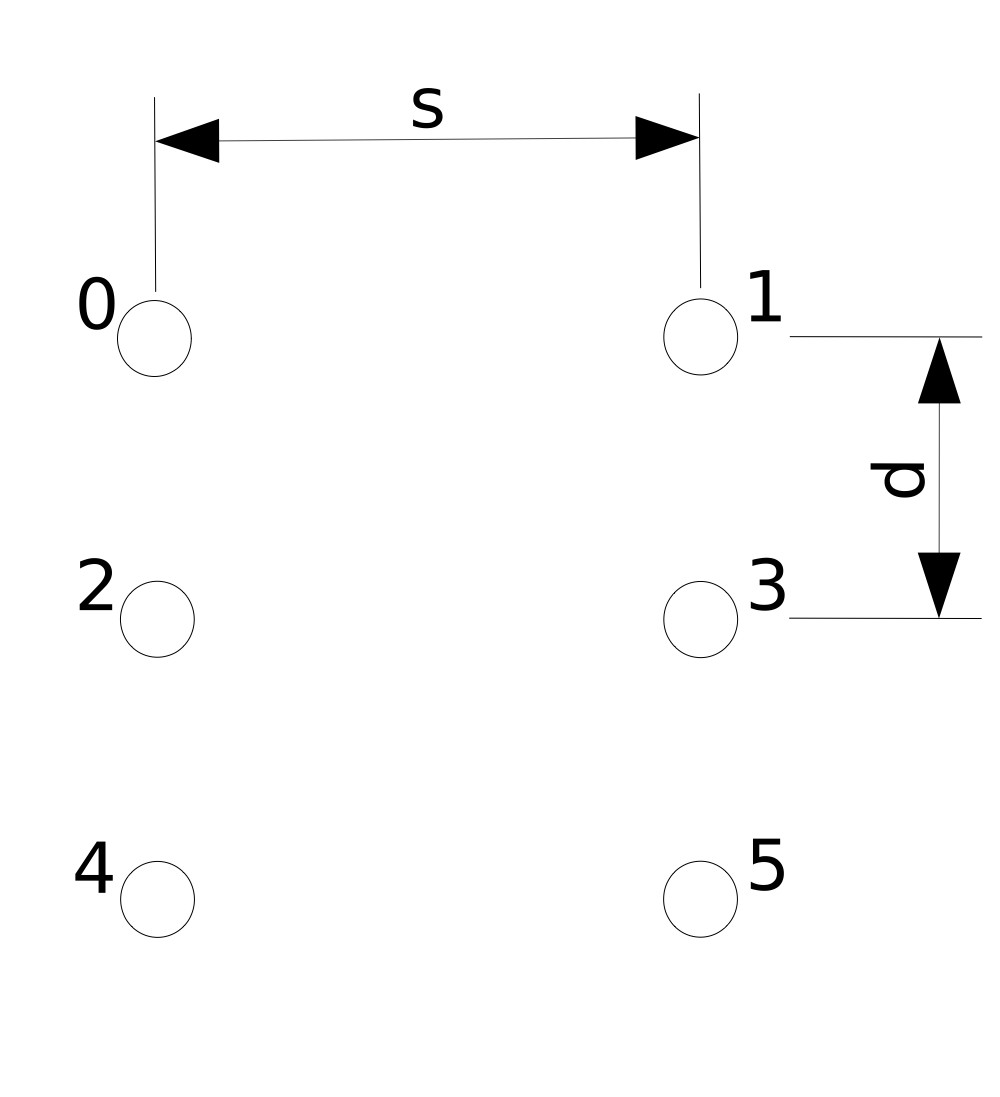
\includegraphics[width=.32\textwidth]{EyeletPattern.png}
	\end{center}
	\caption{Eyelet numbering and dimensions for $N = 3$.}
\end{figure}


When laced, a shoelace of length $L$ will have two free ends for knot tying.
The free length of each end is $f$.  The length of $f$ must fall within a
certain range, $[f_{min}, f_{max}]$ to accommodate a knot that is neither too
small to tie nor so large as to dangle.  See Figure 2 for a common
criss-cross pattern.
\begin{figure}[h]
	\begin{center}
		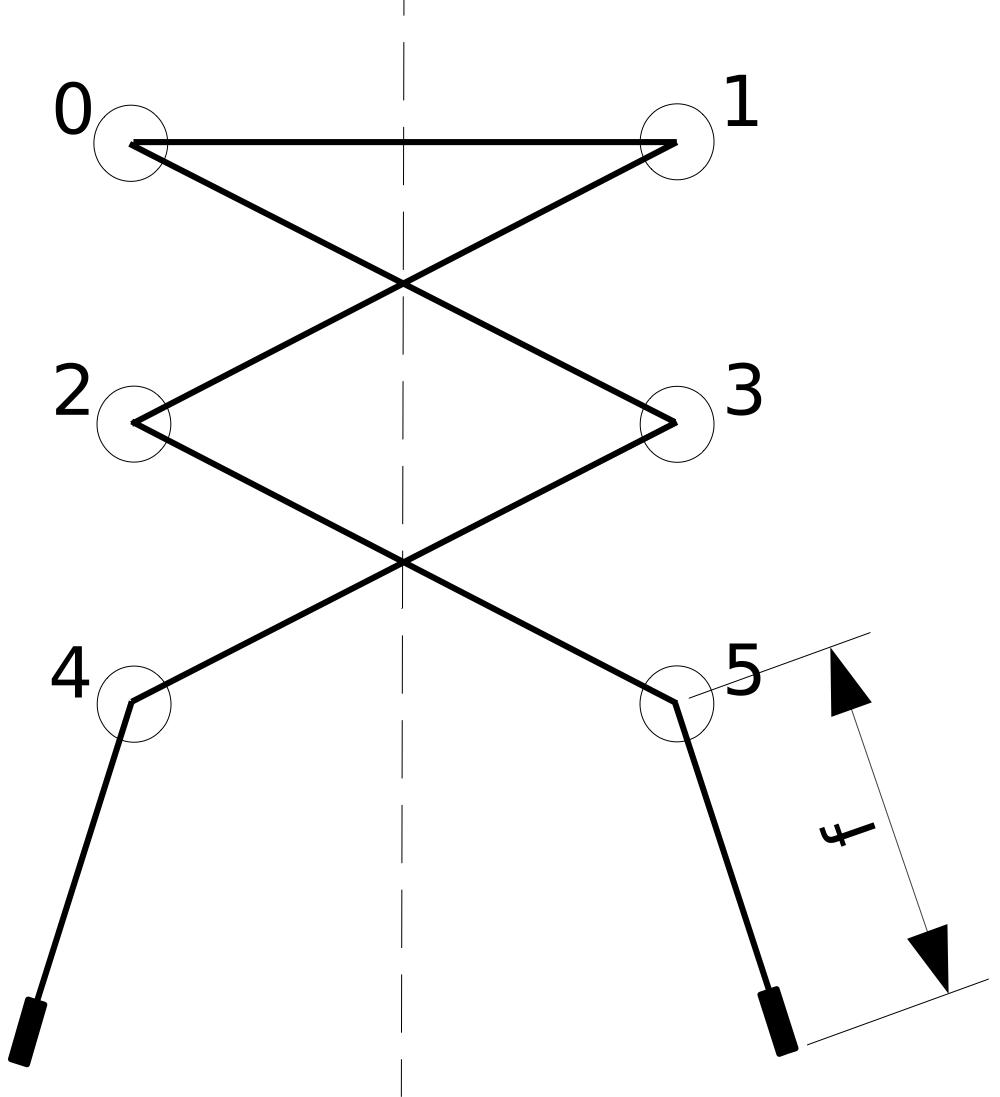
\includegraphics[width=.32\textwidth]{LacingPattern.png}
	\end{center}
	\caption{Criss-cross lacing pattern showing free end length $f$.}
\end{figure}
\par
That special end of a lace that prevents fraying is called an ``aglet.''
You're welcome.
\par
Unfortunately, shoelaces break at the most inopportune times.  Before
purchasing a new shoelace, it is often necessary to retie the shorter, broken
lace, or replace it with another lace borrowed from another shoe.
\par
Given $N, d, s, t, f_{min}, f_{max}$, and a series of replacement shoelace
lengths, $L$, for each shoelace length determine the number of lacing
patterns that leave free ends,
$f$, such that $f_{min} \le f \le f_{max}$.  The rules of lacing are as
follows:
\begin{itemize}
	\item The resulting lacing pattern must be symmetric across a
	line drawn vertically between the even-numbered and odd-numbered eyelets.
	\item The lace can only pass through an eyelet at most once.
	\item The lace can only pass between eyelets in the same
	column that are immediately adjacent.
	\item The free ends of the lace must emerge from eyelet numbers
	$2N - 2$ and $2N - 1$.
	\item The lace must pass directly between eyelet numbers
	0 and 1 to ensure the shoelace holds the shoe on the foot.
\end{itemize}
\par
You are to assume that the surface the eyelets are on is to be treated as
a plane, that the shoelace passes through the center of the eyelets,
and that the thickness of the shoelace itself is negligible.
The total length of the shoelace that is used for lacing is the length
used between the eyelets plus $t$ for each eyelet the shoelace passes
through.  In the example shown in Figure 2, $6t$ of the shoelace length
is used by passing through the six eyelets.

\section*{Input}

The input begins with a single line containing $N, d, s, t, f_{min}, f_{max}$,
separated by whitespace.  Each additional line is a new value of $L$ for which
your program is to count the number of lacing patterns that meet the stated
requirements.  There will be between $1$ and $100$ values of $L$.
All measurements are in integer millimeters.
\par
$N$ will be between $2$ and $9$ inclusive.  $d$ will be between $5$ and $30$ inclusive.
$s$ will be between $10$ and $50$ inclusive.  $t$ will be between $0$ and $4$
inclusive.  $f_{min}$ and $f_{max}$ satisfy $0 \leq f_{min} \leq f_{max} \leq 2\,000$.
Shoelace lengths will be between $200$ and $2\,000$ millimeters
inclusive.  $f_{min}$ and $f_{max}$ will not be within a micron ($0.001$
millimeters) of the free end lengths of a valid lacing pattern.

\section*{Output}

For each shoelace length, your program is to print the number of possible
lacing patterns that meet the above requirements.
Values are to be separated from each other by newlines and/or spaces.

